\section{Visualization Design}

In this section, we first discuss the rationales behind our visualization design. 
Then, we provide a detailed description of the visualization techniques implemented in our system.

%============================================================== Teaser

\begin{figure}[t] 
	\centering
	% \vspace{-4mm}
	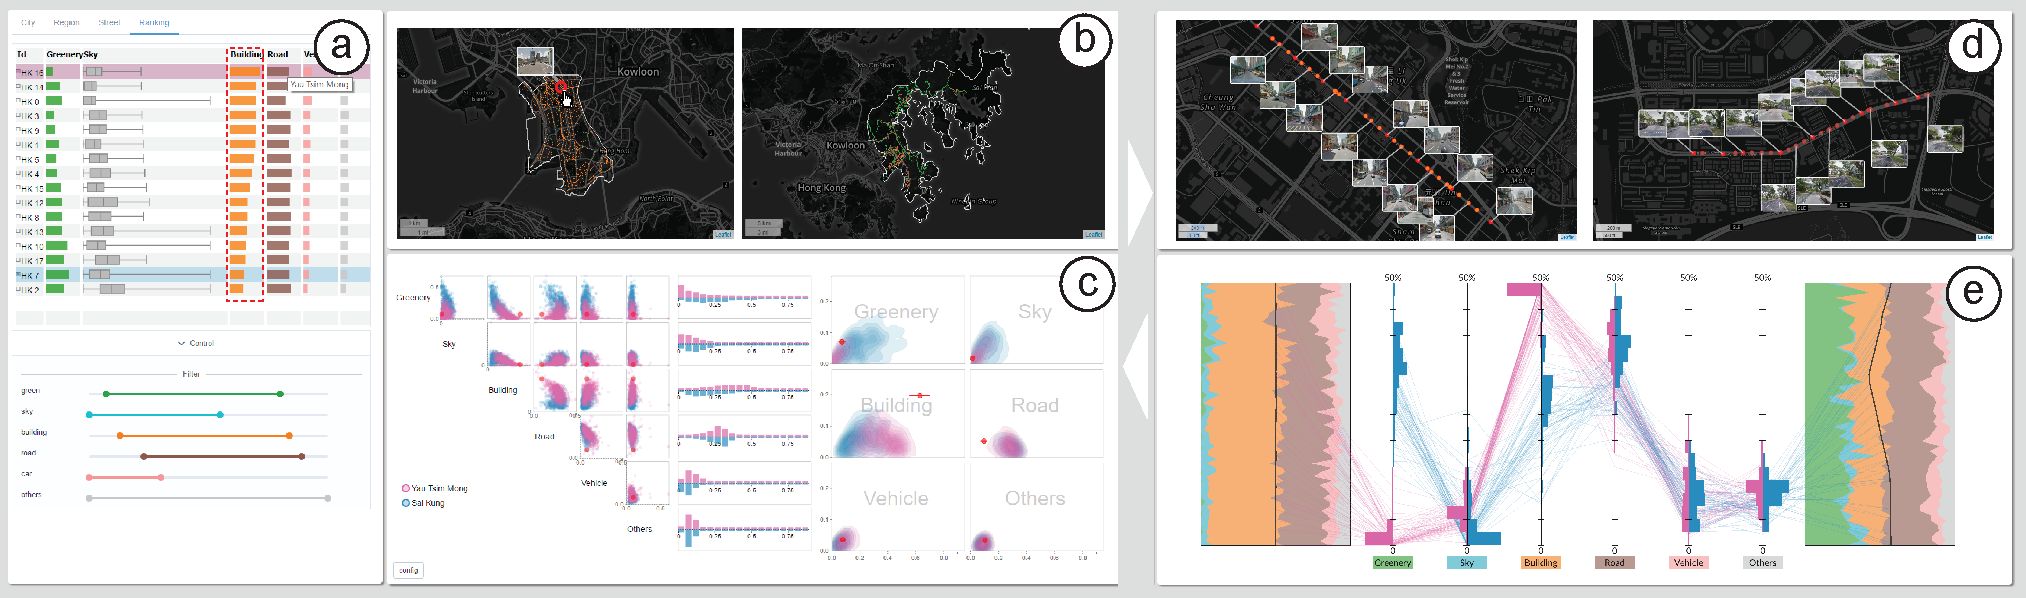
\includegraphics[width=0.98\columnwidth]{figure/streetvizor/fig1_teaser/teaser}
	\vspace{-3mm}
	\caption{StreetVizor system. 
		(a) Control panel enables multi-scale navigation, ranking exploration, and feature filtering.
		(b) Side-by-side map views compare the spatial distribution of human-scale urban forms in two areas-of-interest (AOIs).
		(c) AOI statistic view presents the quantitative measurements, including correlation, histogram, and diversity in the AOIs shown in (b).
		(d) Street map views present detailed street views along two streets.
		(e) Street statistic view extends parallel coordinates with street layouts.}
	\label{fig:c1_teaser}
	\vspace{-1mm}
\end{figure}


%==============================================================

\subsection{Design Rationales}
To address the complex analytical tasks (Section~\ref{ssec:c1_tasks}), a proper visual design should follow the design rationales below:

\begin{enumerate}[label={R.\arabic*:}]

\vspace*{-2mm}
\item
\textbf{Overview+Details}:
To facilitate multi-scale exploration, our system should follow the information-seeking mantra: ``Overview first, zoom and filter, then details on demand"~\cite{shneiderman1996eyes}.
First, the system should provide an overview of human-scale urban forms at city- and region-scales, and then allow users to explore more details at street-scale.
Efficient query and filtering should be provided to enable smooth transitions between these scales.

\vspace*{-2mm}
\item
\textbf{Coordinated Multiple Views}:
Our system should effectively reveal multiple perspectives information of human-scale urban forms, including geographical locations and multivariate features.
CMVs that present linked information and allow users to explore data from multiple joint-perspectives fulfill this requirement.


\vspace*{-2mm}
\item
\textbf{Effective Comparison}:
To enable effective data comparison, different comparative visualization techniques should be employed for multiple-perspective information.
Specifically, given that spatial information for two AOIs/streets is unsuitable for direct overlay, we adopt side-by-side map views.
On the other hand, the feature metric can be mapped on the same scope. 
Therefor, we select a superposition visualization to reveal the differences.

\vspace*{-2mm}
\item
\textbf{Visual Consistency}:
Since multi-scale and multiple-perspective visualizations are to be designed, the system should maintain visual consistency across different visualization modules.
We realize visual consistency by 
1) applying the same layout, i.e., presenting spatial information on the top and quantitative measurements on the bottom, in AOI Explorer and Street Explorer;
2) employing consistent color mappings. 
Specifically, we set green, light blue, orange, brown, light pink, and gray to represent the features of $greenery$, $sky$, $building$, $road$, $vehicle$, and $others$, respectively.
AOIs/streets on the left and right side are colored as red and blue, respectively.

\end{enumerate}

%==============================================================
\subsection{Ranking Explorer}
Ranking Explorer is developed to overview feature attributes across multiple AOI/street candidates to help users quickly identify AOIs/streets for comparison (T.3.1).
The explorer presents each candidate as a row and arranges its multivariate information in seven columns.
The first column provides general information, such as city and region/street id. 
The remaining columns present the six features' mean values as bars, where mean values are normalized and encoded by bar lengths.
Clicking the body of a feature column of interest will expand the column as a boxplot to show statistical distributions.
The explorer also allows users to sort candidates against a particular feature and the ranking will update correspondingly.
Such designs have been well established and evaluated in a previous work~\cite{liu_2017_smartAdP}.

Fig.~\ref{fig:c1_teaser}(a) ranks all districts in Hong Kong in accordance with $building$ feature (red dashed box).
As an example, we observe the detailed statistics of the $sky$ feature.
We select the column for this feature and expand it to boxplot. 
By comparing the orderings of $greenery$, $sky$, and $building$ features, we find $greenery$ and $sky$ features are correlated, while they are negatively correlated with the $building$ feature.
This information helps users narrow down the comparison choices to 1) district HK 16 (Yau Tsim Mong) with the highest $building$ ratio and 2) district HK 7 (Sai Kung) with low $building$ and high $greenery$ ratios, as shown in Figs.~\ref{fig:c1_teaser}(b) \& (c).
% We also find one special region HK 0, which is Central and Western, has both high green feature and building feature. 
% In addition, there is also some street in this region has very high sky feature value. This region could provide a relative good work environment.

% \qm{Even though query methods can effectively help to narrow down to a small scope of AOIs and streets, the planers still need to explore among the small number of candidates. The quantitative ranking and comparison tools based on different features are required for the planers to explore more than two candidates}.
% \qm{The interactions above enable users to narrow down the study scope to several candidates AOIs or streets. To further explore the and find the interested  candidates, we implemented multi-features exploration view (Fig.~\ref{fig:teaser}(a)) which enable quantitative ranking and compare multiple AOIs and streets based on the features interested. Inspired by Lineup~\cite{gratzl2013lineup} and SmartAdp~\cite{liu2017smartadp}, each column indicates one attribute of the AOI/street. The last 6 columns present the six human scale features while other columns present other properties like the id, city they belong to, which can be interactively chosen according to the users' interests. Users can also click on the head to rank the candidates according to the specific features or group several features and rank the candidates by the sum of the selected features.}
%==============================================================
\subsection{AOI Explorer}
\label{ssec:c1_aoi_explorer}
AOI Explorer is developed to provide efficient comparison of human-scale urban forms at city- and region-scales (T.1.1).
The explorer integrates coordinated multiple views, including:

%============================
\subsubsection{AOI Map View}
\label{sssec:c1_aoi_map_view}

We develop side-by-side map views (Figure.~\ref{fig:c1_teaser}(b)) to compare the spatial distributions of human-scale urban forms in two AOIs (T.3.2).
Each map view consists of:
1) a background map layer implemented with Leaflet.js to allow users to change map style (e.g. satellite, street, and sport) for different purposes;
and 2) a point density map overlaid on top of the background map layer, with points representing street views.
The density points are evenly sampled on each street with an upper limit of 10,000 points.
Point color corresponds to the maximum feature value in the street view image.
A corresponding street view image will pop up when the mouse pointer hovers over a point.
Users can select two cities or regions from the navigation panel, or directly manipulate AOIs on the map views with a lasso tool.

Heat map is an alternative design for the point density map.
However, in this work, we focus on the simultaneous analysis of multiple features of human-scale urban forms.
Compositing these features into one heat map~\cite{scheepens_2011_composite} will require redundant user interactions.
In addition, sampling positions are generated along the street network.
Thus, no street views is collected from many places across a city.
In this case, the heat map will generate ambiguity between the two scenarios of 1) no record or 2) low feature values in a region.



%============================
\subsubsection{AOI Statistic View}
\label{sssec:c1_statistic_view}

Besides the map view, which enables the comparison of spatial distributions of human-scale urban forms, we develop AOI Statistic View to allow users to compare various quantitative measurements (T.3.3).
Nonetheless, each AOI may contain too many street views (up to several hundred thousand) that will overload the rendering process.
Moreover, the street views will occlude each other if we simply plot all of them.
To address this problem, we cluster street views into groups based on either their administrative units (districts, divisions, and streets) or a mean-shift clustering algorithm~\cite{comaniciu_2002_meanshift} that works as follows.

\begin{figure}[t]
	\centering
	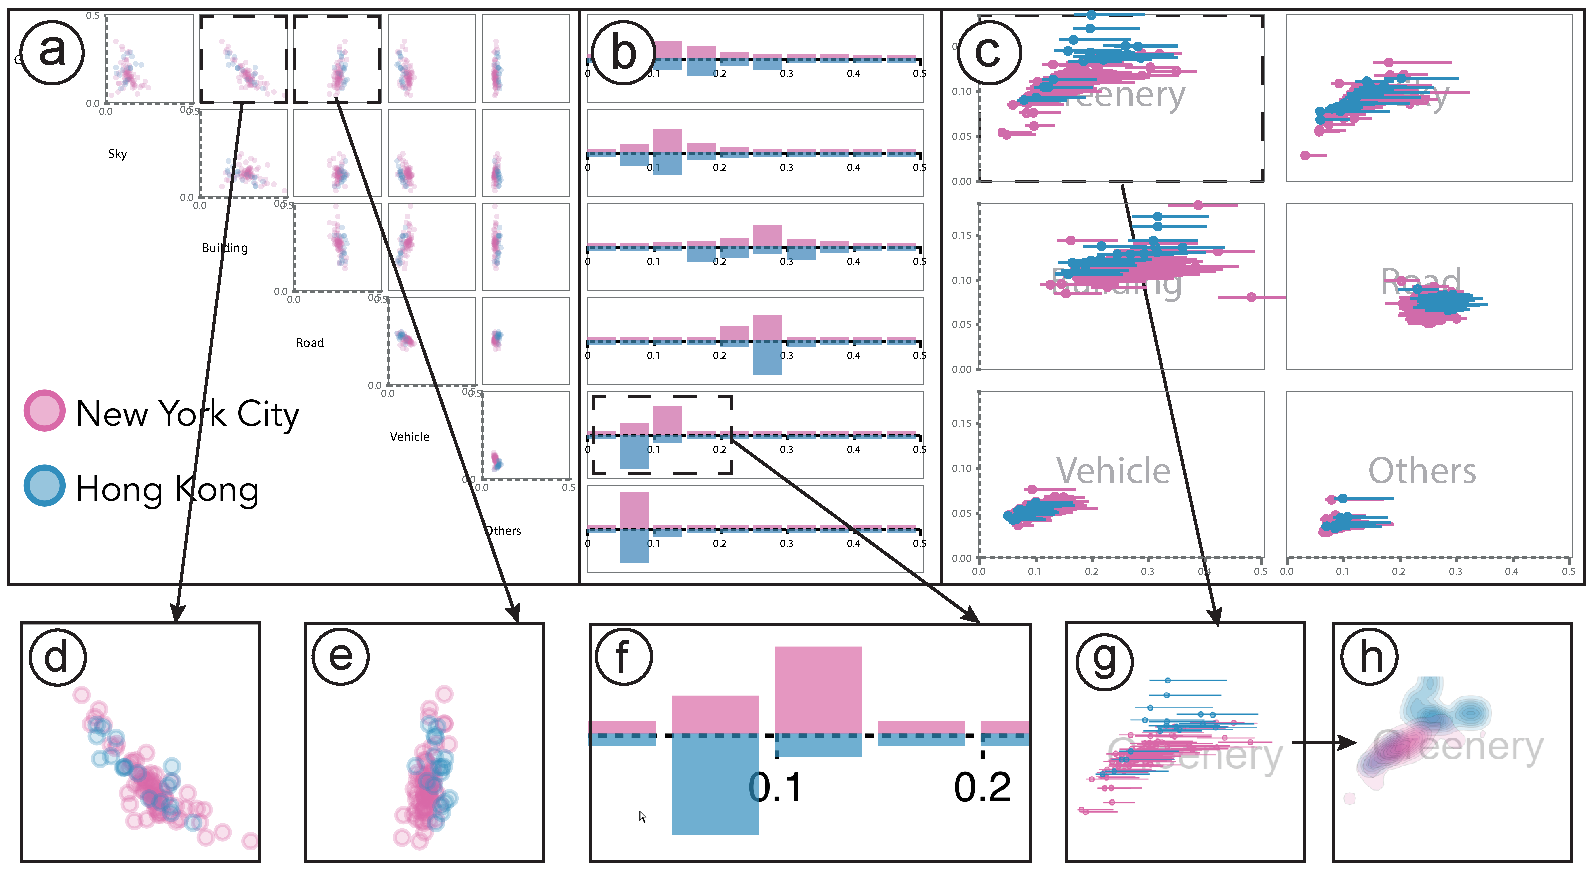
\includegraphics[width=0.9\columnwidth]{figure/streetvizor/fig5_statistic_view/statistic_view}
	\vspace{-4mm}
	\caption{The AOI Statistic View combines (a) a scatterplot matrix to show pair-wise correlations between two features, (b) small multiples of histogram bar charts to overview feature distributions, and (c) small multiples of deviation plots to present feature diversity. }
	\label{fig:c1_statistic_view}
	\vspace{-1mm}
\end{figure}

\vspace*{2mm}
\noindent
\textbf{Mean Shift Clustering}.
We cluster urban forms based on their feature metric and geographical positions.
Our algorithm works in the following way: 
given an input list of $N$ human-scale urban forms \{$UF_{hs}$\}, we first normalize the $lat$ \& $long$ attributes of each $UF_{hs}$ against the boundary of all \{$UF_{hs}$\}.
Then, we combine the normalized $lat_{nor}$ \& $long_{nor}$ with the feature metric to construct a new dataset $X := \{x_1, x_2, ..., x_N\}$, where each data point $x_i$ is in an eight-dimensional space, $R^{8} := \; <lat_{nor}, \; long_{nor}, \; FV_g, \; FV_s, \; FV_b, \; FV_r, \; FV_v, \; FV_o>$.
The distance between two data points is measured as their Euclidean distance.
We then estimate a bandwidth $h$ from $X$, and apply mean-shift clustering algorithm on $X$ using a flat kernel.
Here, the bandwidth estimation and mean shift clustering are performed with a machine learning library \textit{scikit-learn}~\cite{scikit-learn}.
Finally, we generate a list of $m$ urban form clusters $C := \{c_1, c_2, ..., c_m\}$, where each cluster $c_i$ contains $n$ data point $c_i := \{x_1, x_2, ..., x_n\}$.

The clustering process groups geographically close street views with similar feature attributes together.
Given that locations are integrated as two-dimensional spaces, the algorithm forms more local clusters than an algorithm without considering spatial information, which usually generates several big clusters with too many street views.
The algorithm may be further improved by adopting a network-based distance measurement approach other than Euclidean distance.
We expect to form more representative clusters of street views with street network information.
Nonetheless, the current approach fulfills our requirement of reducing visual clutter.

\vspace*{2mm}
After generating the clusters $C$, we further compute and visualize the following quantitative measurements:

\vspace*{-2mm}
\begin{itemize}

\item
\textbf{Feature Correlation}:
We first compute the mean values of the identified features, i.e., \textit{greenery, sky, building, road, vehicle}, and \textit{others} in each cluster $c_i$.
We then plot the pair-wise correlations using a scatterplot matrix (Fig.~\ref{fig:c1_statistic_view}(a)).
Notice that the clusters in the left and right AOIs are colored red and blue, respectively.

\vspace*{-1mm}
\item
\textbf{Feature Histogram}:
Though feature values fall in the range of [0\% - 100\%], we seldom find feature values that exceed 50\%.
Thus, we only consider the range [0\% - 50\%].
For each feature, we divide the range into 10 even parts, i.e., [0\% - 5\%), [5\% - 10\%)..., and aggregate the corresponding value in each street view to each part.
Then, histograms for each feature are plotted as bar charts in an up and down manner for AOIs on the left and right, respectively.
The six histogram bar charts are arranged in small multiples next to the scatterplot matrix (Fig.~\ref{fig:c1_statistic_view}(b)).

\vspace*{-1mm}
\item
\textbf{Feature Diversity}:
We use standard deviation to indicate the measured feature diversity measured for each cluster, and design diversity views that are arranged as six side-by-side small multiples for each feature as shown in Figure~\ref{fig:c1_statistic_view}(c).
In every feature diversity view, each cluster is represented as a dot with its x-value indicating the averaged feature value and y-value indicating standard deviation.
In addition, we use line segments to indicate the largest and smallest feature values in each cluster. 
In case an AOI may have hundreds of clusters that lead to serious visual clutter problem, we implement a contour map view~\cite{chen_2014_visual} (Fig.~\ref{fig:c1_statistic_view}(h)) to show overall distribution patterns.
Users can interactively choose one of the views in accordance with different requirements.

\end{itemize}

The AOI Statistic View comparison of New York City (red) and Hong Kong (blue) is shown in Fig.~\ref{fig:c1_statistic_view}.
From the view, we can easily identify some obvious patterns.
For example, in both cities, \textit{greenery} and \textit{building} features are negatively correlated (Fig.~\ref{fig:c1_statistic_view}(d)).
The correlations between other pairwise features, e.g., \textit{greenery} and \textit{road} (Fig.~\ref{fig:c1_statistic_view}(e)), are not obvious.
From Fig.~\ref{fig:c1_statistic_view}(f), we find that the vehicle ratio is higher in New York City than in Hong Kong.
In addition, we find that although the \textit{greenery} values are similar for both cities, diversity is higher in Hong Kong (Fig.~\ref{fig:c1_statistic_view}(g)).
This results reflects that greenery is better integrated into street space in New York City than in Hong Kong.

%==============================================================
\subsection{Street Explorer}
\label{ssec:c1_street_explorer}

\begin{figure}[t] 
	\centering
	% \vspace{-4mm}
	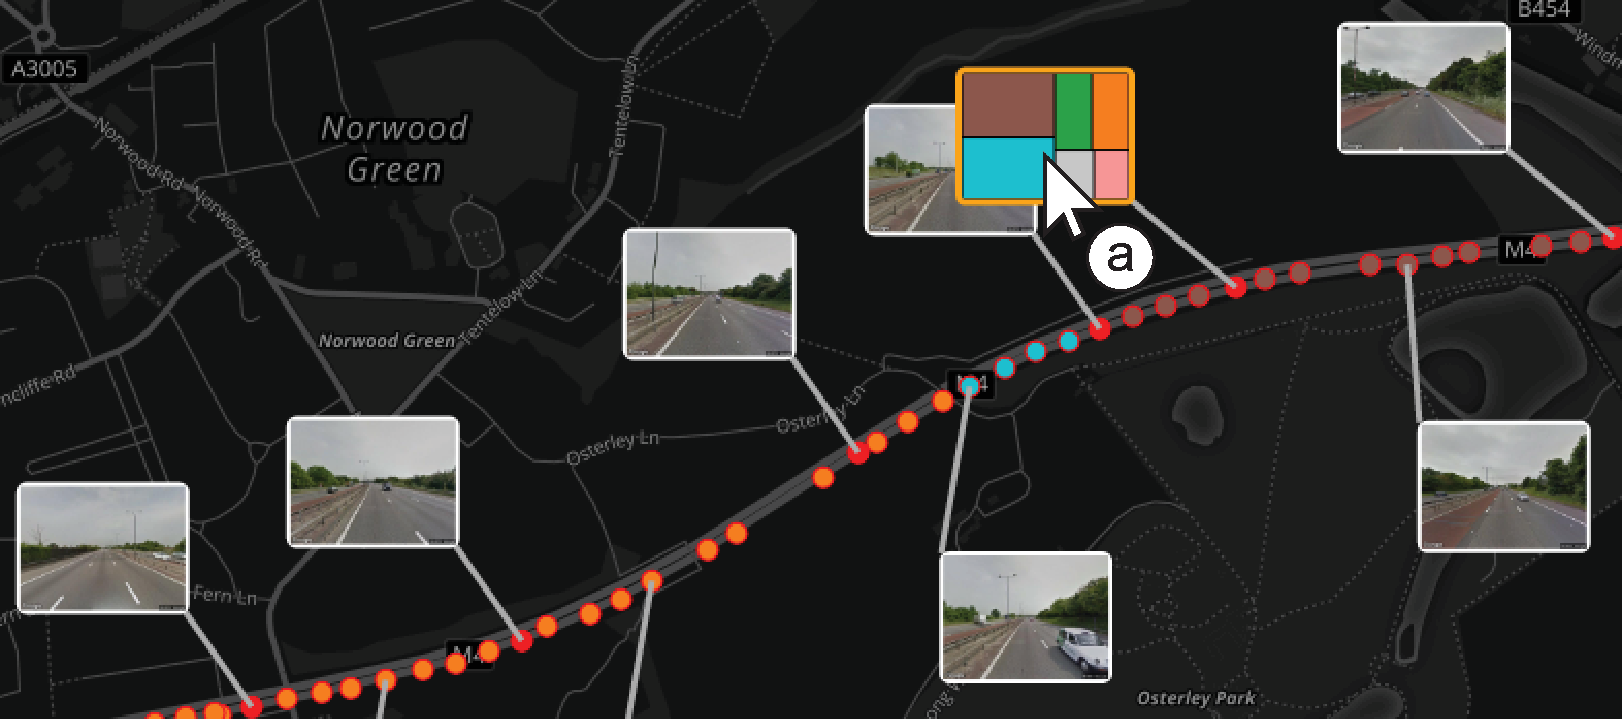
\includegraphics[width=0.9\columnwidth]{figure/streetvizor/fig6_street_map_view/street_map_view}
	\vspace{-3mm}
	\caption{Street Map View provides an overview of all street views along a street as colored points, and highlights images on two sides of the street.
	(a) A tree map showing the feature composition of an image will pop up when the mouse pointer is hovered over the image.}
	\label{fig:c1_street_map}
	\vspace{-1mm}
\end{figure}

%============================

Street Explorer is developed to enable the efficient comparison of human-scale urban forms at street-scale (T.1.2). 
The explorer adapts the same layout as that in the AOI Explorer, i.e., juxtaposition map views are placed on the top of the explorer, whereas detailed statistics view are on the bottom. 

\subsubsection{Street Map View}
\label{sssec:c1_street_view}

Similar to AOI Map View, Street Map View is also developed on top of a background map layer that is implemented using Leaflet.js.
Street views on the street are over-viewed as points with colors that correspond to primary features, i.e., green for $greenery$, light blue for $sky$ and orange for $building$.
In contrast to AOI Map View, Street Map View presents more details of human-scale urban forms by displaying the corresponding street view images along the two sides of a street.
The images are evenly selected in the direction of the street heading. 
In particular, the feature compositions of an image are displayed as a tree map~\cite{shneiderman_1992_tree} when users hover their mouse pointer over the image.
An example is provided in Fig.~\ref{fig:c1_street_map}(a).

%============================

\subsubsection{Street Statistic View}
\label{sssec:c1_street_stat_view}

The design goal for this view is to allow users to quantitatively compare human-scale urban forms from two streets.
Although we can utilize the same views shown in the AOI Statistic View, our collaborating domain expert $SR$ is not satisfied.
$SR$ strongly recommended encoding street layout information in the view, so that users can better leverage their knowledge about streets to perform in-depth analysis.
$SR$ felt the spatial information was not well integrated with the Street Map View.

Based on this goal, we experimented with a few alternative designs and informally evaluated design prototypes with $SR$.
For our first prototype, we designed some glyphs, such as a radial chart or tree map, and directly overlaid the glyphs on the map view.
The design was aborted because isolating statistics on the two maps weakened the effects of comparison.
In addition, such a design easily generated visual clutter, which requires redundant user interactions or clustering to address.
For the second prototype, we encoded street layout information in a similar design as the AOI Statistic View.
However, this method was extremely difficult because the rendering space was fully utilized. 

\begin{figure}[t]
	\centering
	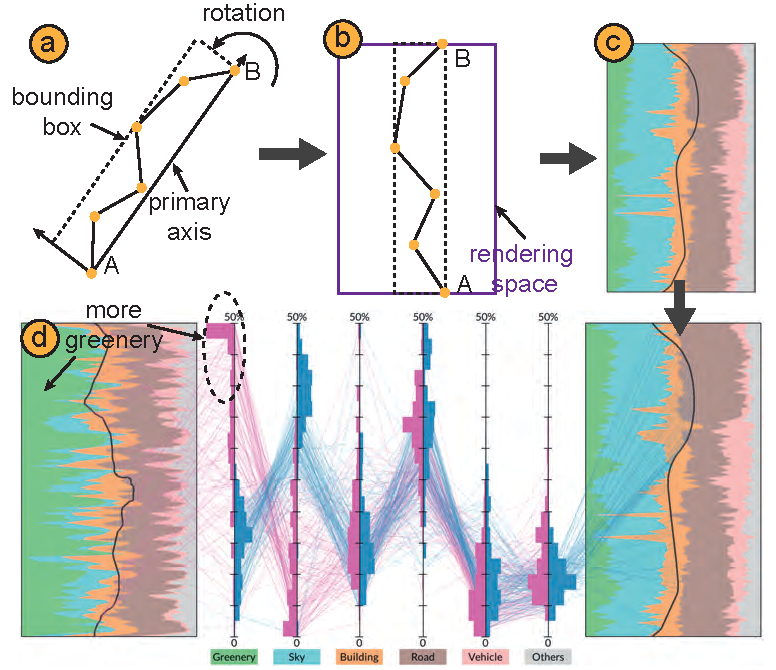
\includegraphics[width=0.9\columnwidth]{figure/streetvizor/fig7_street_model/street_pcp}
	\vspace{-5mm}
	\caption{Overview of the construction process for Street Statistic View:
	(a) Construct minimum bounding box of the street network.
	(b) Rotate the street network such that its bounding box fits in the rendering space.
	(c) Plot themeriver style visualization within the rendering space.
	(d) Enhance parallel coordinates with street layouts on both sides.}
	\label{fig:c1_street_statistic_view}
	\vspace{-1mm}
\end{figure}

\vspace*{2mm}
\noindent
\textbf{PCP with Street Layout}. Inspired by~\cite{qu_2007_visual}, we ultimately develop a design of a parallel coordinates enhanced with street layouts (Fig.~\ref{fig:c1_street_statistic_view}(d)).
We elaborate the construction of this design as follows:

\noindent
\textit{Bounding Box Construction} (Fig.~\ref{fig:c1_street_statistic_view}(a)).
The first step is to construct a minimum bounding box ($MBB$) of the street layout.
% , which is represented as lines connecting positions of corresponding street views.
We find the starting ($A$) and ending ($B$) points, and generate a primary axis pointing from $A$ to $B$.
$MBB$ is generated as the minimum rectangle that contains all nodes of the street network parallel with the primary axis.

\noindent
\textit{Street Layout Rotation} (Fig.~\ref{fig:c1_street_statistic_view}(b)).
Next, we rotate the street layout such that $MBB$ fits in the rendering space, i.e., $A$ and $B$ lay on the top and bottom (or vice versa) sides of the rendering space, and the rotated $MBB$ lays in the center.
In the case that $MBB$ is wider than the rendering space, the street layout outside the rendering space is clipped.
The rotation direction (clockwise or anticlockwise) is determined based on the direction that produces the minimum rotation angle.

\noindent
\textit{ThemeRiver Plotting} (Fig.~\ref{fig:c1_street_statistic_view}(c)).
To fully utilize rendering space, we plot a themeriver-style~\cite{havre_2002_themeriver} visualization to show changes in feature values along a street layout.
Here, the themeriver is plotted in the vertical instead of the traditionally horizontal direction because the street layout is aligned along the y-axis after rotation.
Next, given that street views are sampled evenly along the street layout, we map the street views equally onto the y-axis, i.e., y-values of the themeriver plot reflects the relative positions of street views along the street layout.

We start plotting the themeriver visualization using the left side of the rendering space as the baseline and calculate the upper bound x-values for the $greenery$ feature.
The upper bound x-values of the $greenery$ layer are then used as baseline values for the next feature, i.e., $sky$.
This process is repeated until all features are plotted.
To support better feature comparison, our system allows users to reorder feature sequence by clicking on the feature layer of interest and shifting it to the left side~\cite{byron_2008_stacked}.

\noindent
\textit{PCP Integration} (Fig.~\ref{fig:c1_street_statistic_view}(d)).
The themeriver plot can be used as a coordinate for the PCP.
To enable comparison between two streets, we integrate their themeriver plots into a PCP on left and right sides, and the identified features are used as other coordinates.
Each street view is conveniently presented as a polygonal line, which is colored as red and blue for left and right street views, respectively.
In addition, we aggregate the feature values via binning techniques on left and right sides of each feature coordinate to facilitate the visual comparison of feature distributions.

\vspace*{1mm}
Fig.~\ref{fig:c1_street_statistic_view}(d) presents an example Street Statistic View.
A first glimpse at the two themeriver plots, we can find that the left street contains more $greenery$, while on the right street people can see more $sky$.
This can be found in the distribution comparison on the $greenery$ \& $sky$ coordinates in the middle.
Besides, we can also find that feature values vary dramatically on the left themeriver plot, showing street views are very different along the left street.


\begin{figure}[t]
	\centering
	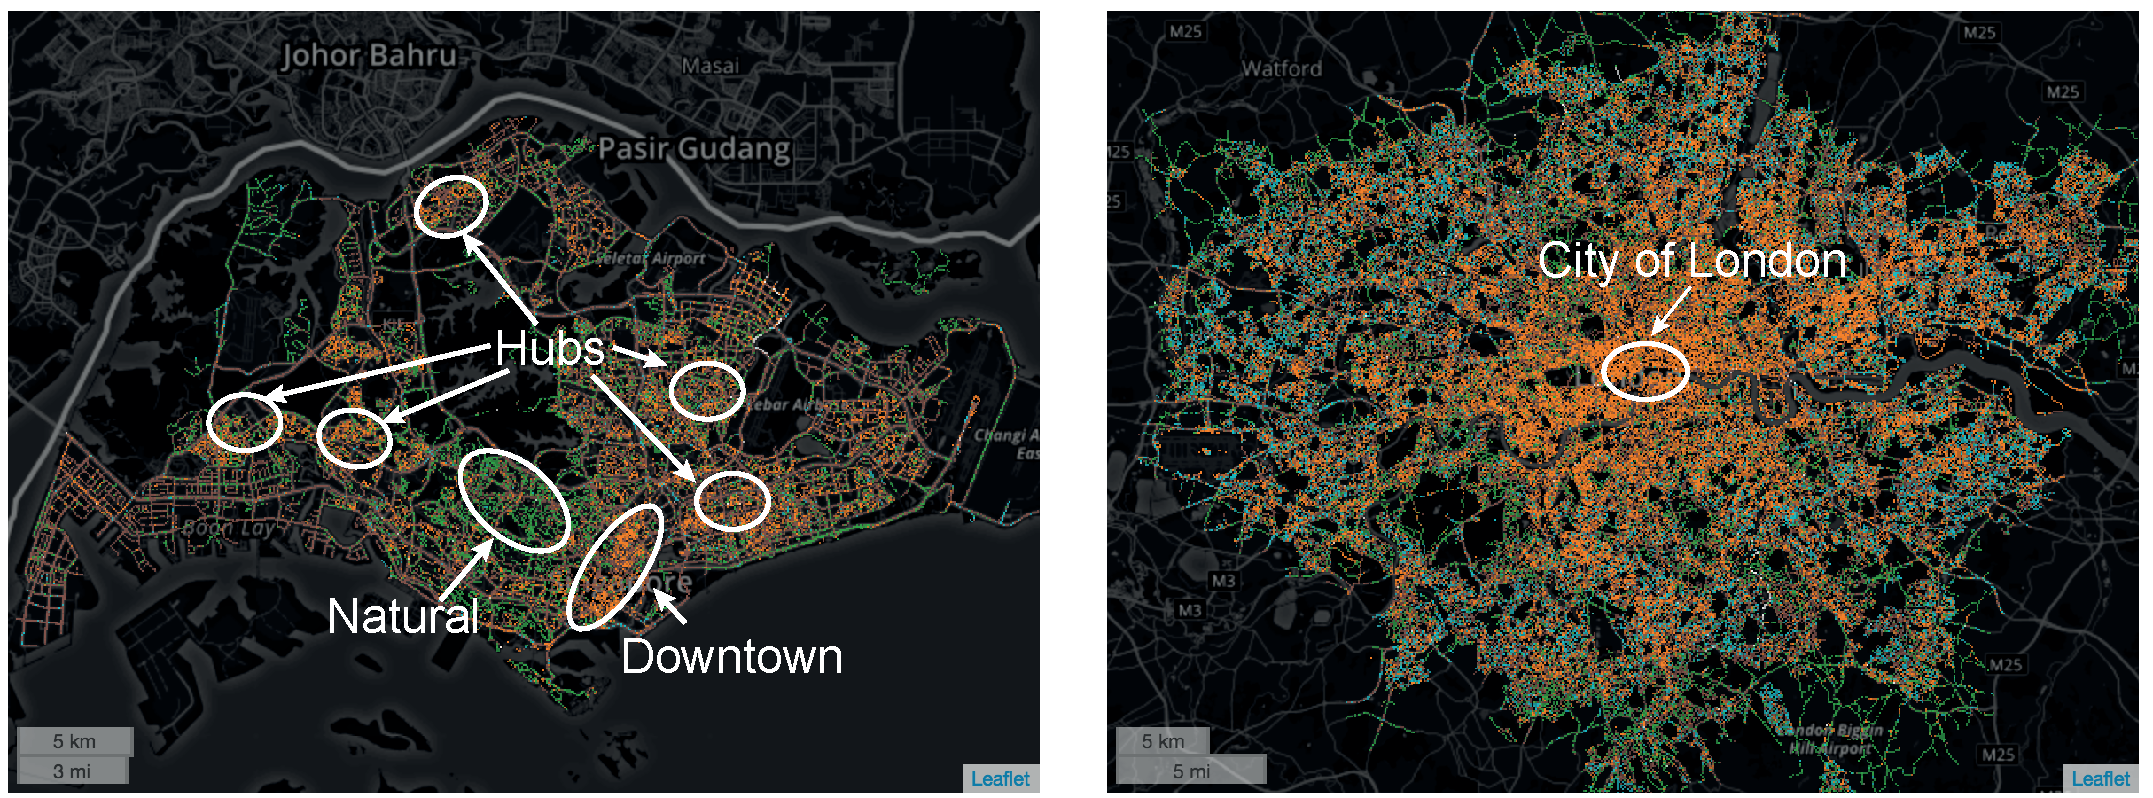
\includegraphics[width=0.95\columnwidth]{figure/streetvizor/fig8_study_1/study_1_spatial}
	\vspace{-4mm}
	\caption{
	AOI Map View compares spatial distributions of human-scale urban forms in Singapore (left) and Greater London (right).
	Orange points (buildings) are concentrated around the highlighted center area of Greater London, i.e., City of London.}
	\label{fig:c1_study_1_spatial}
	% \vspace{-2mm}
\end{figure}




%==============================================================
\subsection{User Interactions}
\label{ssec:c1_user_interaction}

\QM{In addition to basic interactions in each view, StreetVizor also provides a control panel (Fig.~\ref{fig:c1_teaser}(a)) that enables:}

\begin{itemize}

\item
\textit{Multi-scale Navigation}.
To help users navigate effectively across different scales, we develop city-, region- and street-panels.
The city-panel lists all four cities, i.e., Hong Kong, Singapore, Greater London, and New York City.
Users start navigation by selecting a city. 
The region-panel will then list all administrative regions under the city.
For instance, City of London and Kingston will be listed if Greater London is selected.
Similarly, the street-panel lists all the streets inside a selected city or region.
% We also provide a region and street query by entering a corresponding name.

\item
\textit{Feature Filtering}.
Our system also supports filtering human-scale urban forms against a specific feature by specifying the value range with feature sliders. 
By default, each feature slide within [0 - 1], and users can change the minimum and maximum values by dragging the slider buttons.

\end{itemize}

In addition, our system also supports the following user interactions to facilitate visual exploration.
\begin{itemize}

\item
\textit{Details on Demand}.
To enable overview+details (R.1), we develop a set of interactions that allow users to explore the details of human-scale urban forms on demand.
For example, if a street view point is selected in the AOI Map View, the corresponding image will show up.
Thus, users can leverage their domain knowledge by visually examining street views.

\vspace*{-1mm}
\item
\textit{Linking}.
Our system supports automatic linking among the visualization modules in both AOI Explorer and Street Explorer for coordination across multiple views (R.2).
For example, if a specific street view on the AOI Map View is selected, the cluster that contains the street view in the scatterplot matrix and the diversity views will be highlighted accordingly.

\end{itemize}